\documentclass[a4paper,11pt]{article}

\usepackage[german]{babel}
\usepackage[utf8]{inputenc}
\usepackage[T1]{fontenc}
\usepackage{listings}
\usepackage{booktabs}
\usepackage{hyperref}
\usepackage{enumitem}
\usepackage{graphicx}


\title{Programm-Dokumentation: Restaurant-Bestellsystem}
\author{7157747, Gellien, 8425470, Heidusch}
\date{\today}

\begin{document}
\maketitle

\section{Analyse}

\subsection{Aufgabenstellung}
Entwicklung eines Restaurant-Bestellsystems zur Verwaltung von Tischen, Bestellungen und Rechnungen. Das System soll die Möglichkeit bieten, Bestellungen aufzunehmen, zu modifizieren und Rechnungen zu erstellen.

\subsection{Analyse der Problemstellung}
\subsubsection{Ein- und Ausgabe}
\begin{itemize}
    \item Eingabe:
    \begin{itemize}
        \item CSV-Datei mit Speisekarte (food.csv)
        \item Benutzerkommandos über Konsoleneingabe
        \item Tischnummern und Bestellungen
    \end{itemize}

    \item Ausgabe:
    \begin{itemize}
        \item Konsolenausgabe für Menü und Bestellübersicht
        \item Rechnungen als Textdateien (bills.txt)
        \item Statusmeldungen und Fehlermeldungen
    \end{itemize}
\end{itemize}

\subsubsection{Annahmen}
\begin{itemize}
    \item Eindeutige Tischnummern
    \item Gültige Preise (positive Zahlen)
    \item Speisekarte ist im CSV-Format verfügbar
    \item Bestellungen werden pro Tisch gespeichert
\end{itemize}



\subsubsection{Programmstruktur}
\begin{itemize}
    \item Klassen:
    \begin{itemize}
        \item Restaurant: Hauptklasse zur Verwaltung
        \item Menu: Verwaltung der Speisekarte
        \item Table: Verwaltung einzelner Tische
        \item Order: Verwaltung von Bestellungen
        \item OrderItem: Einzelne Bestellposition
    \end{itemize}
    \item Schnittstellen:
    \begin{itemize}
        \item CSV-Datei Interface für Menüverwaltung
        \item Textdatei Interface für Rechnungen
        \item Terminal Interface für die main-loop
    \end{itemize}
\end{itemize}

\section{Coding}
\begin{itemize}
    \item Implementierungssprache: Python 3
    \item Projektstruktur: Modulares Design mit separaten Klassen
    \item Verwendete Bibliotheken: Standard Python Libraries
\end{itemize}

\subsubsection{Befehlsschnittstelle (Command Interface)}
Das System implementiert folgende Hauptbefehle:

\begin{itemize}
    \item \textbf{at (add table)}
    \begin{itemize}
        \item Syntax: at, Tischnummer
        \item Funktion: Fügt einen neuen Tisch mit der angegebenen Nummer hinzu
        \item Beispiel: at, 1
    \end{itemize}

    \item \textbf{aot (add order to table)}
    \begin{itemize}
        \item Syntax: aot, Tischnummer, Speisename, Sonderwunsch
        \item Funktion: Fügt eine neue Bestellung einem bestimmten Tisch hinzu
        \item Beispiel: aot, 1, Pizza, ohne Zwiebeln
    \end{itemize}

    \item \textbf{sb (save bill)}
    \begin{itemize}
        \item Syntax: sb, Tischnummer
        \item Funktion: Speichert die Rechnung für einen bestimmten Tisch in bills.txt
        \item Beispiel: sb, 1
    \end{itemize}

    \item \textbf{rot (remove order from table)}
    \begin{itemize}
        \item Syntax: rot, Tischnummer, Bestellungs-Index
        \item Funktion: Entfernt eine bestimmte Bestellung von einem Tisch
        \item Beispiel: rot, 1, 0
    \end{itemize}

    \item \textbf{asr (add special request)}
    \begin{itemize}
        \item Syntax: asr, Tischnummer, Artikel-Index, Bestellungs-Index, Sonderwunsch
        \item Funktion: Fügt einen Sonderwunsch zu einem bestehenden Bestellartikel hinzu
        \item Beispiel: asr, 1, 0, 0, ohne Zwiebeln
    \end{itemize}

    \item \textbf{Hilfsbefehle}
    \begin{itemize}
        \item h: Zeigt alle verfügbaren Befehle mit Beschreibung an (docstring)
        \item q: Beendet das Programm
    \end{itemize}
\end{itemize}

\subsubsection{Befehlsverarbeitung}
Das System verarbeitet Befehle im Format: ``Befehl, Wert1, Wert2, ...'' und konvertiert die Eingabewerte automatisch in die entsprechenden Datentypen (Integer, Float oder String). Fehlerhafte Befehle werden abgefangen und mit entsprechenden Hinweisen quittiert.


\section{Test}
\subsection{Testfälle}
4 Testfälle wurde beispielsweise in die Dokumentation aufgenommen:\newline
\begin{itemize}
    \item Testfall 1: test\_add\_item
    \begin{itemize}
        \item Äquivalenzklasse: Bestellverwaltung
        \item Test-Typ: Funktional
        \item Repräsentant: Erstellt OrderItem pommes mit Sonderwunsch marmelade
        \item Soll-Ergebnis: item.name == pommes
        \item Kommentar: Prüft korrektes Hinzufügen zur Bestellung
        \item Status: Erfüllt yes
    \end{itemize}
    \item Testfall 2: test\_remove\_item
    \begin{itemize}
        \item Äquivalenzklasse: Bestellverwaltung
        \item Test-Typ: Funktional
        \item Repräsentant: Entfernt Item an Index 0
        \item Soll-Ergebnis: remove\_item(0) == True
        \item Kommentar: Validiert erfolgreiche Entfernung
        \item Status: Erfüllt yes
    \end{itemize}
    \item Testfall 3: test\_add\_table
    \begin{itemize}
        \item Äquivalenzklasse: Tischverwaltung
        \item Test-Typ: Funktional
        \item Repräsentant: Erstellt und verknüpft Bestellkette
        \item Soll-Ergebnis: tables[0] == table
        \item Kommentar: Prüft Integration in Restaurant-Objekt
        \item Status: Erfüllt yes
    \end{itemize}
  \item Testfall 4: test\_add\_order
    \begin{itemize}
        \item Äquivalenzklasse: Tischverwaltung
        \item Test-Typ: Funktional
        \item Repräsentant: Verknüpft Bestellung mit Tisch
        \item Soll-Ergebnis: orders[0] == order
        \item Kommentar: Validiert korrekte Zuordnung
        \item Status: Erfüllt yes
    \end{itemize}
\end{itemize}


\section{UML-Diagramm}
\begin{figure}[h]
    \centering
    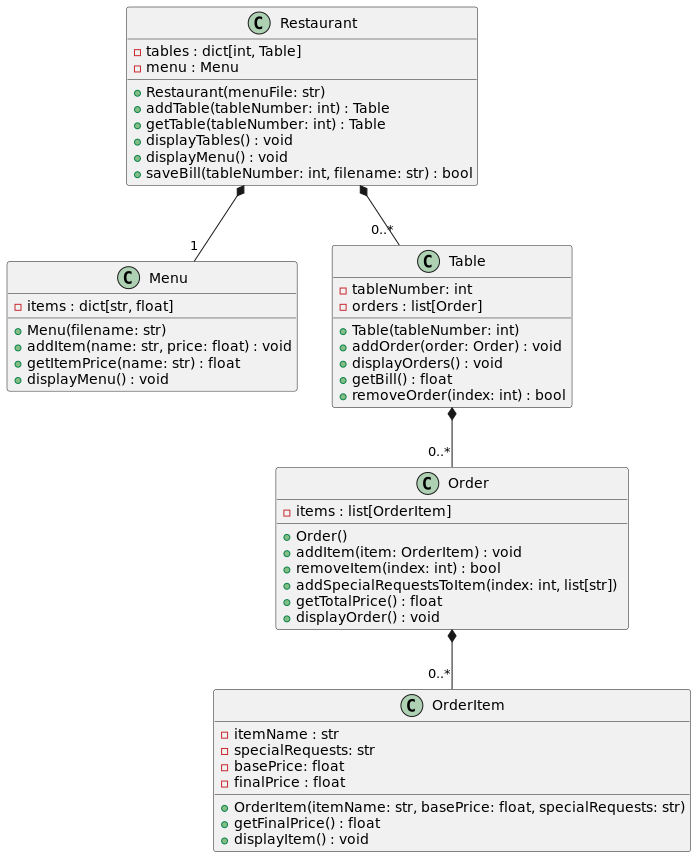
\includegraphics[width=\textwidth]{uml.png}
    \caption{UML-Klassendiagramm des Restaurant-Bestellsyste}
    \label{fig:uml}
\end{figure}

\section{README}
\subsection{Projektbeschreibung}
Restaurant-Bestellsystem zur Verwaltung von Tischen, Bestellungen und Rechnungen in Python.

\subsection{Systemanforderungen}
\begin{itemize}
    \item Python 3.10 oder höher
    \item Standardbibliotheken
    \item Betriebssystem: Plattformunabhängig
\end{itemize}

\subsection{Installation und Bedienung}
\begin{itemize}
    \item Installation:
\begin{itemize}
\item Git Repository klonen bzw. zip-datei öffnen
\item Dependencies installieren:
\begin{verbatim}
pip install -e .
\end{verbatim}
\item Dies installiert das Projekt im Development-Modus mit allen erforderlichen Abhängigkeiten aus der \texttt{setup.py}
\end{itemize}
    \item Startanweisungen:
    \begin{itemize}
        \item Python-Skript aus src/ ausführen
        \item Speisekarte (food.csv) muss vorhanden sein
    \end{itemize}
    \item Bedienungshinweise:
    \begin{itemize}
        \item Tische über Nummer verwalten
        \item Bestellungen pro Tisch aufgeben
        \item Rechnungen über Tischnummer erstellen
    \end{itemize}
\end{itemize}

\subsection{Bekannte Fehler}
Keine bekannten Fehler

\end{document}
